%==============================================================================
%  CHAPTER 13: Generalization and Regularization
%  Part II: Optimization Theory
%==============================================================================
\documentclass[../../main.tex]{subfiles}

\begin{document}

\chapter{Generalization and Regularization}
\label{ch:regularization}

Dropout---randomly turning off neurons during training---sounds absurd. When Hinton first proposed it, reviewers rejected the paper twice. It went on to become one of the most cited papers in deep learning.

\begin{whycare}
Regularization is the difference between a model that memorizes training data and one that generalizes to new data. In production, generalization IS the product. Every percentage point of test accuracy improvement can translate to real business value.
\end{whycare}

\begin{keyconcept}
\textbf{Generalization}\index{generalization|textbf}---the ability to perform well on unseen data---is the central goal of machine learning. \textbf{Regularization}\index{regularization|textbf} constrains or penalizes model complexity to improve generalization. This chapter covers: (1) \textit{explicit regularization penalties} (L1/L2/weight decay), (2) \textit{implicit/structural regularization} (dropout, early stopping), (3) \textit{data augmentation}, and (4) \textit{normalization layers} (BatchNorm, LayerNorm)---which are primarily training stabilizers, though they also affect generalization. Understanding how these distinct techniques work and interact is fundamental to building models that don't just memorize training data.
\end{keyconcept}

\begin{realworld}
\textbf{Why This Matters:} Without regularization, neural networks memorize training data instead of learning patterns.

\textbf{Real Example:} Dropout, introduced by Hinton et al.\ (2012), significantly improved ImageNet results and became widely adopted.

\textbf{Scale:} Large language models typically use modest dropout rates (around 0.1), meaning roughly 10\% of neurons are randomly zeroed during each forward pass.
\end{realworld}

\begin{intuition}[What to Expect]
This chapter proceeds in five parts:
\begin{enumerate}
    \item \textbf{The Problem}: Why models fail to generalize (overfitting, bias-variance tradeoff)
    \item \textbf{Explicit Regularization Penalties}: Terms that directly constrain weights (L1, L2, elastic net, weight decay)
    \item \textbf{Implicit/Structural Regularization}: Techniques that regularize without explicit penalties (dropout, early stopping)
    \item \textbf{Data Augmentation}: Expanding training data through transformations
    \item \textbf{Normalization Layers}: Training stabilizers that also affect generalization (BatchNorm, LayerNorm)
\end{enumerate}
The running theme: \textit{regularization trades training performance for test performance}, and the art lies in finding the right balance.

\textbf{A note on taxonomy:} We discuss normalization layers in this chapter because they affect generalization, but they differ fundamentally from explicit regularization. BatchNorm and LayerNorm are primarily \textit{training stabilizers}---techniques that smooth the optimization landscape and enable faster convergence. While they can have regularization-like side effects (BatchNorm's mini-batch noise acts as implicit regularization), their primary purpose is training stability, not capacity control. We include them here because practitioners must understand how all these techniques interact when building generalizable models.
\end{intuition}

\begin{prerequisites}
\textbf{Before reading this chapter, you should be comfortable with:}
\begin{itemize}
    \item Optimization basics and loss functions (see Book~1, Chapter~8)
    \item Probability and statistics: bias, variance (see Book~1, Chapter~3)
    \item Gradient descent and training loops (Chapter~\ref{ch:gradient-descent})
\end{itemize}
\textbf{Review if needed:} Book~1, Chapter~3 for expectation/variance, Book~1, Chapter~8 for loss minimization
\end{prerequisites}

%------------------------------------------------------------------------------
\section{The Problem: Overfitting and Generalization}
\label{sec:overfitting}

The central challenge of machine learning is not fitting the training data---it is making accurate predictions on \textit{new, unseen data}. This distinction lies at the heart of \textbf{generalization}, as illustrated in Figure~\ref{fig:overfitting-curves}.

\begin{figure}[htbp]
    \centering
    \pdftooltip{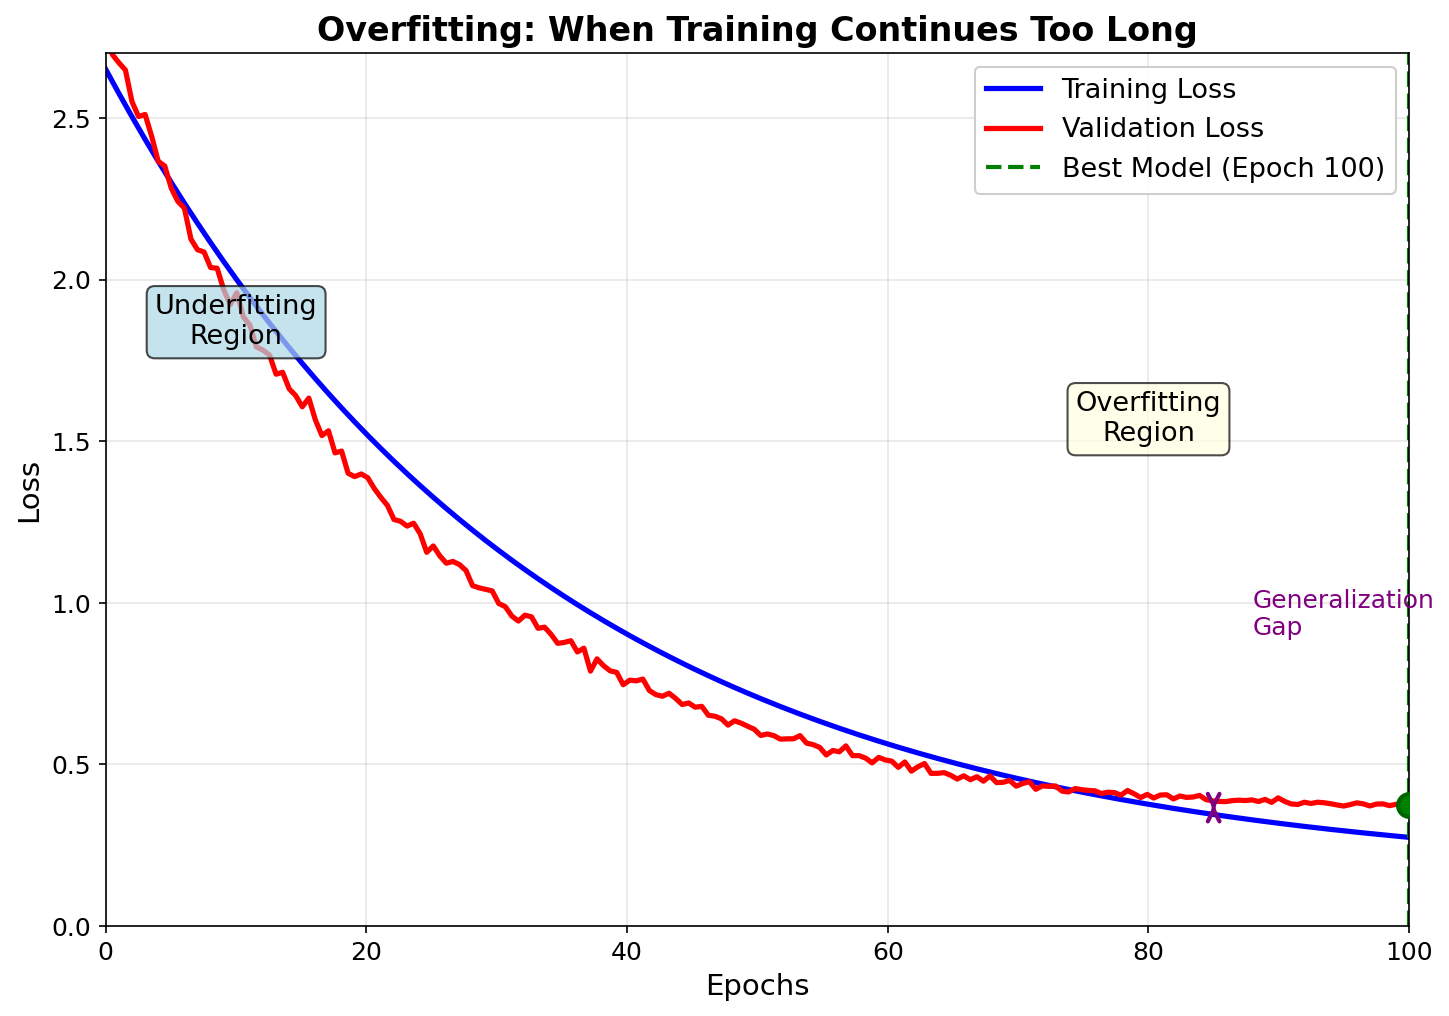
\includegraphics[width=0.85\textwidth]{../../images/diagrams/ch13/overfitting-curves.png}}{Line graph showing loss versus training epochs. The blue training loss curve continuously decreases from high to low values. The red validation loss curve initially decreases alongside training loss, then reaches a minimum and starts increasing, forming a U-shape. A vertical green dashed line marks the epoch where validation loss is minimized, indicating the optimal stopping point.}
    \caption{The classic overfitting signature: training loss (blue) continues to decrease while validation loss (red) increases. The green vertical line marks the optimal stopping point. Training beyond this point memorizes noise rather than learning patterns.}
    \label{fig:overfitting-curves}
\end{figure}

\begin{definition}{Overfitting}{overfitting-def}
\textbf{Overfitting}\index{overfitting|textbf} occurs when a model learns the training data too well, capturing noise and idiosyncrasies specific to that particular dataset. An overfit model exhibits low training error but high test error.
\end{definition}

\begin{definition}{Underfitting}{underfitting-def}
\textbf{Underfitting}\index{underfitting|textbf} occurs when a model is too simple to capture the underlying structure. An underfit model exhibits high error on both training and test data.
\end{definition}

\begin{intuition}
Consider fitting a polynomial to noisy data points. A low-degree polynomial (linear or quadratic) might underfit, failing to capture the true curvature. A very high-degree polynomial passes through every training point but oscillates wildly between them. The goal is to find the ``sweet spot''---complex enough to capture the true pattern but simple enough to avoid memorizing noise.
\end{intuition}

%------------------------------------------------------------------------------
\section{The Bias-Variance Tradeoff}
\label{sec:bias-variance}

The bias-variance decomposition formalizes the tradeoff between model complexity and generalization.

\begin{theorem}{Expected Prediction Error}{expected-error}
For a new input $\vect{x}$ with true output $y = f^*(\vect{x}) + \epsilon$, the expected squared prediction error decomposes as:
\[
    \E\left[(y - \hat{f}(\vect{x}))^2\right] = \underbrace{\E\left[(\hat{f} - \E[\hat{f}])^2\right]}_{\text{Variance}} + \underbrace{(\E[\hat{f}] - f^*)^2}_{\text{Bias}^2} + \underbrace{\sigma^2}_{\text{Irreducible}}
\]
where expectations are over training data and noise.
\end{theorem}

\begin{definition}{Bias and Variance}{bias-variance-def}
\textbf{Bias} measures how far the average prediction is from truth: $\text{Bias} = \E[\hat{f}(\vect{x})] - f^*(\vect{x})$. \textbf{Variance} measures sensitivity to training data: $\text{Var} = \E[(\hat{f} - \E[\hat{f}])^2]$.
\end{definition}

\begin{principle}
\textbf{The Bias-Variance Tradeoff:}\index{bias-variance tradeoff|textbf} Simple models have high bias but low variance; complex models have low bias but high variance. The optimal model minimizes total error by balancing these competing sources. Regularization increases bias (constrains the model) but decreases variance (reduces sensitivity to training data). When variance dominates, this tradeoff reduces total error.
\end{principle}

\begin{important}
\textbf{A Modern Caveat: Double Descent and Overparameterized Models}

The classical bias-variance tradeoff assumes you cannot reduce both bias and variance simultaneously---increasing model complexity trades one for the other, producing the familiar U-shaped test error curve.

Modern deep learning challenges this view. Very large neural networks exhibit \textbf{double descent}\index{double descent|textbf}: as model complexity increases past the interpolation threshold (where the model can perfectly fit training data), test error first rises (as expected), but then \textit{decreases again} for even larger models. Extremely overparameterized models can achieve both low bias AND low variance.

\textbf{What this means for practitioners:}
\begin{itemize}
    \item The classical U-shaped curve is not wrong---it describes behavior up to the interpolation threshold
    \item Beyond that threshold, implicit regularization from SGD, architecture choices, and optimization dynamics enable large models to generalize well
    \item This does NOT mean ``regularization is obsolete''---regularization still helps, and the double descent phenomenon depends on proper optimization
    \item The practical implication: don't be afraid of large models if you have the compute, but also don't assume bigger is always better without proper training
\end{itemize}

Double descent is an active research area. The key takeaway: the classical bias-variance tradeoff remains useful intuition, but modern deep learning operates in a regime where additional complexity (and implicit regularization) can sometimes reduce both bias and variance.
\end{important}

\begin{example}{Bias-Variance in House Price Prediction}{ch13-bias-variance-example}
Suppose we train 10 models on different samples to predict a house worth \$500K:
\begin{itemize}
    \item Predictions: \$480K, \$520K, \$490K, \$510K, \$485K, \$515K, \$495K, \$505K, \$488K, \$512K
    \item Mean prediction: \$500K (unbiased---matches true value)
    \item Variance: spread of predictions around the mean ($\approx$\$15K standard deviation)
\end{itemize}
A high-bias model might consistently predict \$450K (wrong but stable). A high-variance model might predict anywhere from \$300K to \$700K (unstable). Regularization reduces variance at the cost of introducing some bias.
\end{example}

%------------------------------------------------------------------------------
\section{Regularized Loss Functions}
\label{sec:regularized-loss}

Regularization typically adds a penalty term to the loss function:

\begin{definition}{Regularized Objective}{regularized-objective-def}
A \textbf{regularized objective function} takes the form:
\[
    \mathcal{L}_{\text{reg}}(\vect{\theta}) = \mathcal{L}_{\text{data}}(\vect{\theta}) + \lambda \Omega(\vect{\theta})
\]
where $\mathcal{L}_{\text{data}}$ is the data-fitting term, $\Omega(\vect{\theta})$ measures complexity, and $\lambda \geq 0$ controls regularization strength.
\end{definition}

\begin{intuition}
The regularization term acts as a ``preference'' for simpler models. We accept slightly worse training error in exchange for better generalization. Setting $\lambda = 0$ gives no regularization; $\lambda \to \infty$ produces the simplest possible model.
\end{intuition}

%------------------------------------------------------------------------------
\section{Regularization as Modified Optimization}
\label{sec:regularization-optimization}

Understanding regularization from an optimization perspective reveals its fundamental nature: \textbf{regularization modifies what we optimize}, not just how we optimize it.

\begin{keyconcept}
\textbf{Three Views of Regularization:}
\begin{enumerate}
    \item \textbf{Explicit penalty (loss modification):} Add a term to the objective: $\min_{\vect{\theta}} \mathcal{L}_{\text{data}}(\vect{\theta}) + \lambda\Omega(\vect{\theta})$. This directly changes the loss landscape, creating new minima that balance data fit against model complexity.

    \item \textbf{Implicit from algorithm:} Some optimization algorithms inherently favor certain solutions without explicit penalties. SGD with small learning rates finds flatter minima; early stopping limits how far parameters drift from initialization. The algorithm \textit{is} the regularizer.

    \item \textbf{Architectural constraint:} The model structure itself constrains the hypothesis space. Convolutions enforce translation equivariance; skip connections bias toward identity mappings; weight sharing in RNNs limits effective parameters. Architecture encodes inductive bias.
\end{enumerate}
These three views are complementary: a well-regularized model typically combines explicit penalties, algorithmic choices, and architectural constraints.
\end{keyconcept}

\begin{intuition}
Consider the original optimization problem: $\min_{\vect{\theta}} \mathcal{L}_{\text{data}}(\vect{\theta})$. This finds parameters that best fit the training data---but ``best fit'' often means memorization. The regularized problem $\min_{\vect{\theta}} \mathcal{L}_{\text{data}}(\vect{\theta}) + \lambda\Omega(\vect{\theta})$ changes the question from ``what fits best?'' to ``what fits well while remaining simple?'' The regularization strength $\lambda$ controls how much we value simplicity over fit.
\end{intuition}

\begin{principle}
\textbf{Regularization shifts the optimization target.} Without regularization, we seek the global minimum of $\mathcal{L}_{\text{data}}$. With regularization, we seek a different point---one that may have higher training loss but lower total regularized loss. This new optimum typically generalizes better because it represents a simpler model that captures patterns rather than noise.
\end{principle}

%------------------------------------------------------------------------------
\section{L2 Regularization (Ridge)}
\label{sec:l2-regularization}

\begin{definition}{L2 Regularization}{l2-reg-def}
\textbf{L2 regularization}\index{L2 regularization|textbf}\index{Ridge regression|see{L2 regularization}}\index{Tikhonov regularization|see{L2 regularization}} (ridge or Tikhonov regularization) penalizes squared parameter magnitudes:
\[
    \mathcal{L}_{\text{ridge}}(\vect{\theta}) = \mathcal{L}_{\text{data}}(\vect{\theta}) + \frac{\lambda}{2}\norm{\vect{\theta}}_2^2 = \mathcal{L}_{\text{data}}(\vect{\theta}) + \frac{\lambda}{2}\sum_{j=1}^{p} \theta_j^2
\]
\end{definition}

\begin{theorem}{Constrained Optimization View}{l2-constrained}
L2 regularization is equivalent to constrained optimization:
\[
    \min_{\vect{\theta}} \mathcal{L}_{\text{data}}(\vect{\theta}) \quad \text{subject to} \quad \norm{\vect{\theta}}_2^2 \leq c
\]
for some $c$ depending on $\lambda$. Larger $\lambda$ means smaller $c$, forcing parameters closer to zero.
\end{theorem}

\begin{intuition}
Geometrically, L2 regularization restricts parameters to lie within a spherical region centered at the origin. The constraint boundary is smooth, so optimal solutions tend to have all parameters nonzero but small.
\end{intuition}

\subsection{Ridge Regression}

For linear regression with squared error loss, L2 regularization yields a closed-form solution.

\begin{theorem}{Ridge Regression Solution}{ridge-solution}
For the objective $\mathcal{L}(\vect{w}) = \norm{\mat{X}\vect{w} - \vect{y}}_2^2 + \lambda\norm{\vect{w}}_2^2$, the optimal weights are:
\[
    \vect{w}_{\text{ridge}} = (\mat{X}\trans\mat{X} + \lambda\mat{I})^{-1}\mat{X}\trans\vect{y}
\]
\end{theorem}

\begin{keyconcept}
The term $\lambda\mat{I}$ ensures $\mat{X}\trans\mat{X} + \lambda\mat{I}$ is always invertible, even when $\mat{X}\trans\mat{X}$ is singular (e.g., more features than samples). This is why ridge regression is called \textbf{regularized least squares}.
\end{keyconcept}

\begin{theorem}{SVD Perspective}{ridge-svd}
Let $\mat{X} = \mat{U}\mat{\Sigma}\mat{V}\trans$ be the SVD. The ridge prediction is:
\[
    \hat{\vect{y}}_{\text{ridge}} = \sum_{j=1}^{r} \frac{\sigma_j^2}{\sigma_j^2 + \lambda} (\vect{u}_j\trans \vect{y})\vect{u}_j
\]
The factor $\frac{\sigma_j^2}{\sigma_j^2 + \lambda}$ shrinks components with small singular values (weak signal) more than those with large singular values (strong signal).
\end{theorem}

%------------------------------------------------------------------------------
\section{L1 Regularization (Lasso)}
\label{sec:l1-regularization}

\begin{definition}{L1 Regularization}{l1-reg-def}
\textbf{L1 regularization}\index{L1 regularization|textbf}\index{Lasso|textbf}\index{sparsity|textbf} (Lasso: Least Absolute Shrinkage and Selection Operator) penalizes absolute values:
\[
    \mathcal{L}_{\text{lasso}}(\vect{\theta}) = \mathcal{L}_{\text{data}}(\vect{\theta}) + \lambda\norm{\vect{\theta}}_1 = \mathcal{L}_{\text{data}}(\vect{\theta}) + \lambda\sum_{j=1}^{p} |\theta_j|
\]
\end{definition}

\begin{theorem}{L1 Induces Sparsity}{l1-sparsity}
L1 regularization produces \textbf{sparse} solutions where many parameters are exactly zero, effectively performing automatic feature selection.
\end{theorem}

\begin{intuition}
Geometrically, L1 constrains parameters to a diamond-shaped region (an $\ell_1$-ball). The diamond has corners along the axes, and the optimal solution often occurs at these corners where some coordinates are zero. In contrast, L2's spherical constraint has no corners.
\end{intuition}

\begin{aha}
L1 makes weights exactly zero; L2 makes them small but non-zero. Geometrically: L1's diamond-shaped constraint has corners on the axes (sparse solutions); L2's circle doesn't touch axes (dense solutions). That's why L1 does feature selection.
\end{aha}

This geometric distinction is shown in Figure~\ref{fig:l1-vs-l2}.

\begin{figure}[htbp]
    \centering
    \pdftooltip{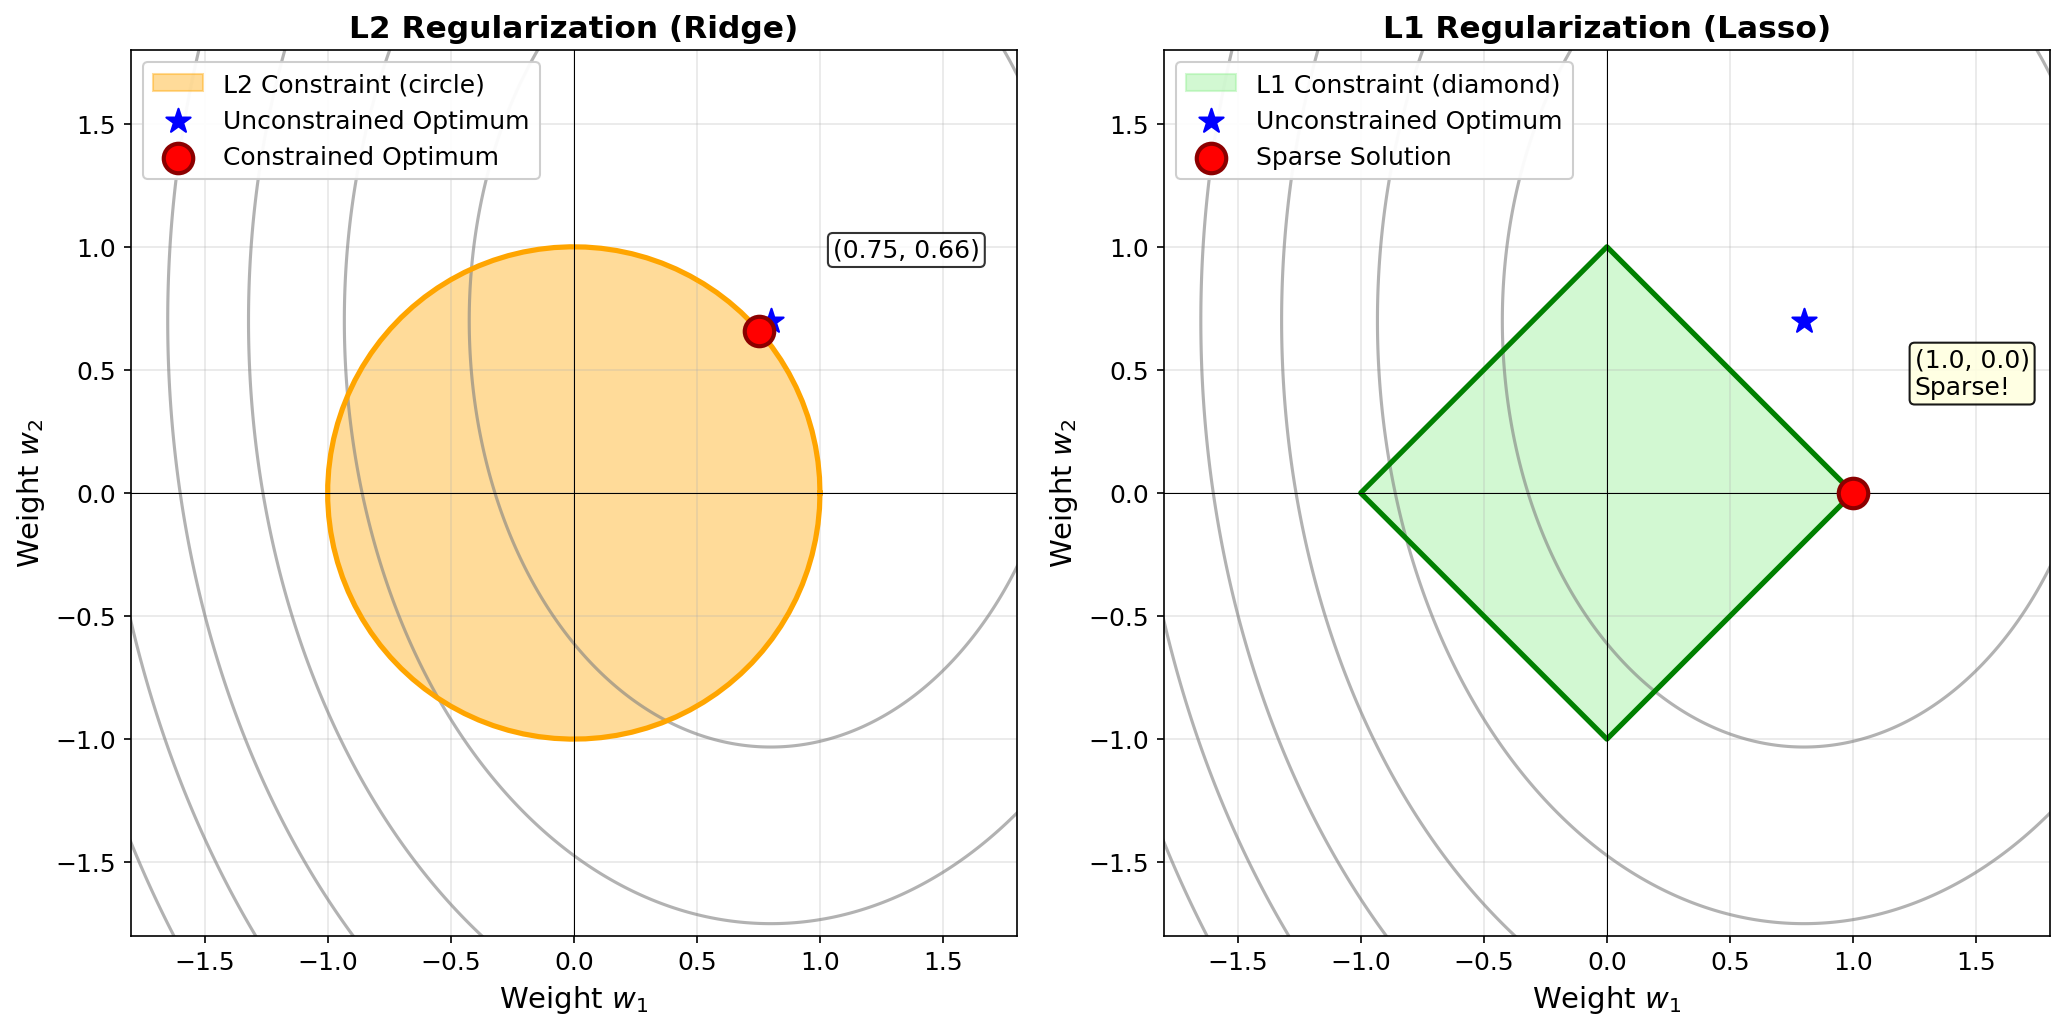
\includegraphics[width=0.95\textwidth]{../../images/diagrams/ch13/l1-vs-l2.png}}{Side-by-side comparison of L1 and L2 regularization geometry. Left panel shows L2: elliptical contour lines representing the loss function intersect with a circular constraint region centered at the origin. The optimal point lies on the circle boundary away from the axes. Right panel shows L1: the same elliptical contours intersect with a diamond-shaped (rotated square) constraint region. The optimal point lies at a corner of the diamond on one of the axes, where one coordinate equals zero.}
    \caption{Geometric intuition for L1 vs L2 regularization. Left: L2's circular constraint rarely touches the axes, producing dense solutions. Right: L1's diamond constraint has corners on the axes, producing sparse solutions with many weights exactly zero.}
    \label{fig:l1-vs-l2}
\end{figure}

\begin{commonmistakes}
\begin{itemize}
    \item \textbf{Mistake:} Thinking more regularization is always better for generalization

    \textbf{Why it's wrong:} Over-regularization causes \emph{underfitting}---the model becomes too simple to capture true patterns. There is an optimal regularization strength that balances bias and variance.

    \textbf{Correct understanding:} Regularization trades training error for test error. Too little $\Rightarrow$ overfitting (low train, high test error). Too much $\Rightarrow$ underfitting (high train \emph{and} test error). Use validation to find the sweet spot.
\end{itemize}
\end{commonmistakes}

\begin{example}{L1 vs L2 Geometry}{l1-l2-geometry-ex}
Minimize $f(\theta_1, \theta_2) = (\theta_1 - 1)^2 + (\theta_2 - 1)^2$ with constraints:
\begin{itemize}
    \item \textbf{L2}: $\theta_1^2 + \theta_2^2 \leq c$ (circle). Solution typically nonzero in both coordinates.
    \item \textbf{L1}: $|\theta_1| + |\theta_2| \leq c$ (diamond). Solution often at a corner with one coordinate zero.
\end{itemize}
\end{example}

\begin{definition}{Soft Thresholding}{soft-threshold-def}
The proximal operator\index{proximal operator} for L1 is the \textbf{soft thresholding}\index{soft thresholding|textbf} operator:
\[
    S_\lambda(\theta) = \sign(\theta) \cdot \max(|\theta| - \lambda, 0)
\]
\end{definition}

\begin{pythoncode}
import numpy as np

def soft_threshold(theta, lambda_reg):
    """Apply soft thresholding (L1 proximal operator)."""
    return np.sign(theta) * np.maximum(np.abs(theta) - lambda_reg, 0)

def lasso_coordinate_descent(X, y, lambda_reg, max_iters=1000, tol=1e-6):
    """Lasso regression via coordinate descent."""
    m, p = X.shape
    w = np.zeros(p)
    for _ in range(max_iters):
        w_old = w.copy()
        for j in range(p):
            residual = y - X @ w + X[:, j] * w[j]
            rho_j = X[:, j] @ residual
            if np.sum(X[:, j]**2) > 0:
                w[j] = soft_threshold(rho_j, lambda_reg * m) / np.sum(X[:, j]**2)
        if np.linalg.norm(w - w_old) < tol:
            break
    return w
\end{pythoncode}

%------------------------------------------------------------------------------
\section{Elastic Net}
\label{sec:elastic-net}

\begin{definition}{Elastic Net}{elastic-net-def}
\textbf{Elastic net}\index{elastic net|textbf} combines L1 and L2 regularization:
\[
    \Omega_{\text{elastic}}(\vect{\theta}) = \alpha\norm{\vect{\theta}}_1 + \frac{1-\alpha}{2}\norm{\vect{\theta}}_2^2
\]
with mixing parameter $\alpha \in [0,1]$.
\end{definition}

\begin{keyconcept}
\textbf{When to use each:}
\begin{itemize}
    \item \textbf{L2 (Ridge)}: All features believed relevant; stability needed
    \item \textbf{L1 (Lasso)}: Sparsity desired; feature selection
    \item \textbf{Elastic Net}: Correlated features (Lasso arbitrarily selects one)
\end{itemize}
Elastic net's L2 component encourages correlated features to have similar weights (``grouping effect''), while L1 provides sparsity.
\end{keyconcept}

%------------------------------------------------------------------------------
\section{Weight Decay vs L2 Regularization}
\label{sec:weight-decay}

\begin{definition}{Weight Decay}{weight-decay-def}
\textbf{Weight decay}\index{weight decay|textbf} modifies the gradient descent update directly:
\[
    \vect{\theta}_{t+1} = (1 - \eta\lambda)\vect{\theta}_t - \eta\grad\mathcal{L}(\vect{\theta}_t)
\]
The factor $(1 - \eta\lambda)$ ``decays'' weights toward zero each step.
\end{definition}

\begin{theorem}{Equivalence for SGD}{weight-decay-l2-equiv}
For standard SGD, weight decay and L2 regularization are equivalent. Adding $\frac{\lambda}{2}\norm{\vect{\theta}}_2^2$ to the loss produces gradient $\grad\mathcal{L} + \lambda\vect{\theta}$, giving the same update.
\end{theorem}

\begin{important}
\textbf{For adaptive optimizers (Adam, RMSprop), weight decay and L2 regularization are NOT equivalent!} With L2 in Adam, the regularization gradient $\lambda\vect{\theta}$ gets scaled by adaptive learning rates. True weight decay (AdamW) applies decay directly, maintaining consistent regularization.
\end{important}

\begin{checkpoint}
What's the relationship between L2 regularization and weight decay? Are they always equivalent?
\end{checkpoint}

\begin{pythoncode}
class AdamW:
    """Adam with decoupled weight decay."""
    def __init__(self, lr=0.001, beta1=0.9, beta2=0.999, eps=1e-8, wd=0.01):
        self.lr, self.beta1, self.beta2 = lr, beta1, beta2
        self.epsilon, self.weight_decay = eps, wd
        self.m = self.v = None
        self.t = 0

    def update(self, params, grads):
        if self.m is None:
            self.m, self.v = np.zeros_like(params), np.zeros_like(params)
        self.t += 1
        self.m = self.beta1 * self.m + (1 - self.beta1) * grads
        self.v = self.beta2 * self.v + (1 - self.beta2) * grads**2
        m_hat = self.m / (1 - self.beta1**self.t)
        v_hat = self.v / (1 - self.beta2**self.t)
        # Decoupled weight decay: apply to pre-update params in single step
        adam_update = m_hat / (np.sqrt(v_hat) + self.epsilon)
        return params * (1 - self.lr * self.weight_decay) - self.lr * adam_update
\end{pythoncode}

%------------------------------------------------------------------------------
\section{Implicit and Structural Regularization}
\label{sec:implicit-structural}

The techniques in this section regularize models without adding explicit penalty terms to the loss function. Instead, they modify the training procedure or architecture in ways that improve generalization.

%------------------------------------------------------------------------------
\subsection{Dropout}
\label{sec:dropout}

\begin{warstory}
\textbf{The Paper Nobody Wanted}

In 2012, Hinton and his students proposed dropout: randomly setting neurons to zero during training. The idea seemed absurd. Reviewers at NIPS rejected the paper---twice.

``Randomly destroying information can't possibly help,'' they argued. ``This has no theoretical justification.''

Srivastava, Hinton, Krizhevsky, Sutskever, and Salakhutdinov eventually published in JMLR in 2014. The paper has become one of the most cited in machine learning history. Dropout became standard practice in deep learning.

The theoretical understanding came later: dropout is approximately equivalent to training an ensemble of exponentially many networks that share weights. It also acts as a form of adaptive regularization.

\textbf{Lesson:} Sometimes the best ideas sound crazy at first. Empirical results matter. If something works consistently, pursue understanding---but don't let lack of theory stop you from trying bold ideas.
\end{warstory}

\begin{definition}{Dropout}{dropout-def}
\textbf{Dropout}\index{dropout|textbf}~\cite{srivastava2014dropout} randomly sets a fraction $p$ of neurons to zero during training:
\[
    \tilde{\vect{h}} = \vect{m} \odot \vect{h}, \quad m_i \sim \text{Bernoulli}(1-p)
\]
where $\vect{m}$ is a binary mask and $p$ is the dropout probability.
\end{definition}

\begin{theorem}{Dropout as Ensemble}{dropout-ensemble}
Dropout trains an exponentially large ensemble of $2^n$ ``thinned'' networks that share parameters. At test time, using all units (with scaled weights) approximates the ensemble average.
\end{theorem}

\begin{checkpoint}
Why does dropout work? Explain it as approximate ensemble averaging.
\end{checkpoint}

\begin{important}
\textbf{Training vs Inference:} During training, apply dropout (random masking). At inference, no dropout---scale activations by $(1-p)$. \textbf{Inverted dropout}\index{inverted dropout|textbf} scales by $1/(1-p)$ during training so no scaling is needed at inference: during training, each neuron's output is kept with probability $(1-p)$, so without scaling the expected output would be $(1-p) \cdot h$. Scaling by $1/(1-p)$ during training ensures the expected training output equals the test-time output (when all neurons are active).

\textbf{Common mistake:} Applying dropout at test time. Dropout should only be active during training. PyTorch's \texttt{nn.Dropout} automatically disables when \texttt{model.eval()} is called, but custom implementations must check \texttt{self.training}.
\end{important}

\begin{pythoncode}
def dropout_forward(x, dropout_prob, training=True):
    """
    Forward pass with inverted dropout.

    Inverted dropout: scale during training, not inference.
    The 1/(1-p) factor compensates for dropped neurons so that
    expected activation magnitude stays constant. This means
    no adjustment is needed at inference time.
    """
    if not training or dropout_prob == 0:
        return x, None
    keep_prob = 1 - dropout_prob
    # Scale by 1/keep_prob to maintain expected value
    mask = (np.random.rand(*x.shape) < keep_prob) / keep_prob
    return x * mask, mask

def dropout_backward(dout, mask):
    """Backward pass for dropout."""
    return dout * mask if mask is not None else dout
\end{pythoncode}

\begin{intuition}
Dropout prevents \textbf{co-adaptation}\index{co-adaptation}---neurons learn to be useful independently rather than relying on specific other neurons being present. Like training a team where any member might be absent.
\end{intuition}

\textbf{Variants}: Spatial Dropout (drops feature maps in CNNs), DropConnect (drops weights), Variational Dropout (same mask across time steps for RNNs).

\begin{realworld}
\textbf{BERT's Layered Dropout Strategy}

When Google developed BERT~\cite{devlin2019bert}, they employed a carefully tuned \textbf{layer-specific dropout strategy} that became a template for Transformer models.

BERT uses three distinct dropout rates: (1) \textbf{Attention dropout} (0.1) applied to attention weights after softmax, preventing over-reliance on specific token relationships; (2) \textbf{Hidden dropout} (0.1) applied after each sub-layer (attention and feed-forward), regularizing intermediate representations; (3) \textbf{Embedding dropout} (0.1) applied to input embeddings, preventing memorization of specific token patterns.

The insight was that different components require different regularization. Attention heads can easily memorize training patterns---specific word pairs that always co-occur. Hidden layers are more robust but still benefit from regularization. Embeddings need dropout to prevent the model from memorizing surface patterns rather than learning semantic relationships.

This layered approach improved BERT's generalization on downstream tasks compared to uniform dropout. Other large language models use similar or lower dropout rates, though configurations vary by architecture and scale.

\textbf{Lesson:} Regularization is not one-size-fits-all. Different model components have different overfitting risks and benefit from targeted dropout strategies.
\end{realworld}

%------------------------------------------------------------------------------
\section{Normalization Layers: Training Stabilizers}
\label{sec:normalization-layers}

\begin{important}
\textbf{Normalization vs. Regularization:} While normalization layers can have regularization-like effects, their primary purpose is \textit{training stability}, not regularization. BatchNorm and LayerNorm smooth the loss landscape, enable higher learning rates, and reduce sensitivity to initialization. Any regularization effect is secondary---a byproduct of the normalization mechanism, not the design goal. We include them in this chapter because understanding their interaction with true regularizers is essential for building models that generalize well.
\end{important}

%------------------------------------------------------------------------------
\subsection{Batch Normalization}
\label{sec:batch-norm}

\begin{definition}{Batch Normalization}{batch-norm-def}
\textbf{Batch normalization}\index{batch normalization|textbf}\index{BatchNorm|see{batch normalization}}~\cite{ioffe2015batch} normalizes layer inputs across the mini-batch:
\[
    \hat{x}_i = \frac{x_i - \mu_\mathcal{B}}{\sqrt{\sigma_\mathcal{B}^2 + \epsilon}}, \quad y_i = \gamma \hat{x}_i + \beta
\]
where $\mu_\mathcal{B} = \frac{1}{m}\sum_{i=1}^m x_i$ and $\sigma_\mathcal{B}^2 = \frac{1}{m}\sum_{i=1}^m (x_i - \mu_\mathcal{B})^2$ are batch statistics, and $\gamma, \beta$ are learnable scale and shift parameters.
\end{definition}

\begin{keyconcept}
\textbf{Why BatchNorm works (multiple perspectives):}
\begin{enumerate}
    \item \textbf{Primary effect---Training stability:} Reduces internal covariate shift (stabilizes layer input distributions)
    \item \textbf{Primary effect---Optimization:} Smooths the loss landscape, enabling larger learning rates
    \item \textbf{Secondary effect---Implicit regularization:} Adds noise through batch statistics (but this is a side effect, not the goal)
    \item Decouples direction and magnitude of activations
\end{enumerate}
\end{keyconcept}

\begin{algorithm}[htbp]
\caption{Batch Normalization: Training}
\label{alg:batchnorm-train}
\begin{algorithmic}[1]
\Require Mini-batch $\mathcal{B} = \{x_1, \ldots, x_m\}$, parameters $\gamma, \beta$, small $\epsilon$
\Ensure Normalized outputs $\{y_1, \ldots, y_m\}$
\State $\mu_\mathcal{B} \gets \frac{1}{m}\sum_{i=1}^m x_i$ \Comment{Batch mean}
\State $\sigma_\mathcal{B}^2 \gets \frac{1}{m}\sum_{i=1}^m (x_i - \mu_\mathcal{B})^2$ \Comment{Batch variance}
\State $\hat{x}_i \gets \frac{x_i - \mu_\mathcal{B}}{\sqrt{\sigma_\mathcal{B}^2 + \epsilon}}$ for all $i$ \Comment{Normalize}
\State $y_i \gets \gamma \hat{x}_i + \beta$ for all $i$ \Comment{Scale and shift}
\State Update: $\mu_{\text{run}} \gets \alpha\mu_{\text{run}} + (1-\alpha)\mu_\mathcal{B}$
\State Update: $\sigma^2_{\text{run}} \gets \alpha\sigma^2_{\text{run}} + (1-\alpha)\sigma^2_\mathcal{B}$
\State \Return $\{y_i\}$
\end{algorithmic}
\end{algorithm}

Note: PyTorch's \texttt{momentum} parameter equals $(1-\alpha)$ in this notation. With PyTorch's default \texttt{momentum=0.1}, we have $\alpha=0.9$.

\begin{important}
\textbf{Training vs Inference:} During training, use batch statistics $\mu_\mathcal{B}, \sigma^2_\mathcal{B}$. At inference, use running (population) statistics $\mu_{\text{run}}, \sigma^2_{\text{run}}$ for deterministic outputs.

\textbf{Common bug:} Forgetting to call \texttt{model.eval()} before inference. In training mode, BatchNorm uses batch statistics (stochastic); in eval mode, it uses accumulated running statistics (deterministic). Failing to switch modes causes inconsistent predictions and degraded accuracy at test time.
\end{important}

\begin{pythoncode}
class BatchNorm:
    """Batch normalization layer."""
    def __init__(self, num_features, momentum=0.1, epsilon=1e-5):
        self.gamma = np.ones(num_features)
        self.beta = np.zeros(num_features)
        self.epsilon, self.momentum = epsilon, momentum
        self.running_mean = np.zeros(num_features)
        self.running_var = np.ones(num_features)

    def forward(self, x, training=True):
        if training:
            mean, var = x.mean(axis=0), x.var(axis=0)
            self.running_mean = (1-self.momentum)*self.running_mean + self.momentum*mean
            self.running_var = (1-self.momentum)*self.running_var + self.momentum*var
        else:
            mean, var = self.running_mean, self.running_var
        x_norm = (x - mean) / np.sqrt(var + self.epsilon)
        return self.gamma * x_norm + self.beta
\end{pythoncode}

%------------------------------------------------------------------------------
\subsection{Layer Normalization}
\label{sec:layer-norm}

\begin{definition}{Layer Normalization}{layer-norm-def}
\textbf{Layer normalization}\index{layer normalization|textbf}\index{LayerNorm|see{layer normalization}} normalizes across features for each sample:
\[
    \hat{x}_i = \frac{x_i - \mu_i}{\sqrt{\sigma_i^2 + \epsilon}}
\]
where $\mu_i, \sigma_i^2$ are computed over the feature dimension for sample $i$.
\end{definition}

\begin{keyconcept}
\textbf{BatchNorm vs LayerNorm:}
\begin{center}
\begin{tabular}{lll}
\toprule
\textbf{Aspect} & \textbf{BatchNorm} & \textbf{LayerNorm} \\
\midrule
Normalization axis & Across batch & Across features \\
Batch size dependency & Yes & No \\
Typical use & CNNs & Transformers, RNNs \\
Inference behavior & Uses running stats & Same as training \\
\bottomrule
\end{tabular}
\end{center}
LayerNorm is essential for Transformers due to variable sequence lengths.
\end{keyconcept}

\textbf{Other methods}: Instance Normalization\index{instance normalization} (per-channel per-sample, for style transfer), Group Normalization\index{group normalization|textbf} (channel groups, for small batches), RMSNorm\index{RMSNorm|textbf} (LayerNorm without mean centering):
\[
    \text{RMSNorm}: \hat{x} = \frac{x}{\sqrt{\frac{1}{d}\sum_{j=1}^d x_j^2 + \epsilon}}
\]
RMSNorm~\cite{zhang2019rmsnorm} is increasingly preferred in large language models (LLaMA, Gemma, Mistral) because removing mean-centering offers computational savings with negligible accuracy impact. Prefer RMSNorm for efficiency-critical transformer training.

%------------------------------------------------------------------------------
\section{Data Augmentation}
\label{sec:data-augmentation}

\begin{definition}{Data Augmentation}{data-aug-def}
\textbf{Data augmentation}\index{data augmentation|textbf} expands training data with label-preserving transformations, encoding prior knowledge about invariances.
\end{definition}

\begin{principle}
If a cat remains a cat when flipped horizontally, train on both original and flipped images. The model learns the invariance instead of memorizing specific pixel patterns.
\end{principle}

\textbf{Image augmentation}:
\begin{itemize}
    \item \textbf{Geometric}: Rotation, flipping, cropping, scaling
    \item \textbf{Photometric}: Brightness, contrast, saturation, hue
    \item \textbf{Occlusion}: Cutout\index{cutout|textbf} (random rectangles), random erasing\index{random erasing}
    \item \textbf{Mixing}: Mixup, CutMix\index{CutMix}
\end{itemize}

\begin{definition}{Mixup}{mixup-def}
\textbf{Mixup}\index{mixup|textbf} interpolates training pairs: $\tilde{\vect{x}} = \lambda \vect{x}_i + (1-\lambda)\vect{x}_j$, $\tilde{y} = \lambda y_i + (1-\lambda)y_j$ where $\lambda \sim \text{Beta}(\alpha, \alpha)$.
\end{definition}

\begin{pythoncode}
def mixup(x1, y1, x2, y2, alpha=0.2):
    """Apply mixup augmentation."""
    if alpha <= 0:
        raise ValueError(f"alpha must be positive, got {alpha}")
    lam = np.random.beta(alpha, alpha)
    return lam * x1 + (1 - lam) * x2, lam * y1 + (1 - lam) * y2

def cutout(image, mask_size):
    """Apply cutout (random rectangular mask)."""
    h, w = image.shape[:2]
    mask_size = min(mask_size, h, w)  # Ensure cutout fits
    cy, cx = np.random.randint(h), np.random.randint(w)
    y1, y2 = np.clip([cy - mask_size//2, cy + mask_size//2], 0, h)
    x1, x2 = np.clip([cx - mask_size//2, cx + mask_size//2], 0, w)
    image_aug = image.copy()
    image_aug[y1:y2, x1:x2] = 0
    return image_aug
\end{pythoncode}

\textbf{Text augmentation}: Synonym replacement, random insertion/swap/deletion, back-translation.

%------------------------------------------------------------------------------
\section{Early Stopping}
\label{sec:early-stopping}

\begin{definition}{Early Stopping}{early-stopping-def}
\textbf{Early stopping}\index{early stopping|textbf} halts training when validation performance stops improving.
\end{definition}

\begin{algorithm}[htbp]
\caption{Early Stopping}
\label{alg:early-stopping}
\begin{algorithmic}[1]
\Require Training/validation data, patience $k$, model $\vect{\theta}_0$
\Ensure Best model $\vect{\theta}^*$
\State $\vect{\theta}^* \gets \vect{\theta}_0$, best\_loss $\gets \infty$, wait $\gets 0$
\For{epoch $= 1, 2, \ldots$}
    \State Train one epoch, evaluate $\mathcal{L}_{\text{val}}$
    \If{$\mathcal{L}_{\text{val}} < \text{best\_loss}$}
        \State best\_loss $\gets \mathcal{L}_{\text{val}}$, $\vect{\theta}^* \gets \vect{\theta}$, wait $\gets 0$
    \Else
        \State wait $\gets$ wait + 1
        \If{wait $\geq k$}
            \State \textbf{break}
        \EndIf
    \EndIf
\EndFor
\State \Return $\vect{\theta}^*$
\end{algorithmic}
\end{algorithm}

\begin{theorem}{Early Stopping as L2 Regularization}{early-stopping-l2}
For linear models with gradient descent from zero initialization, early stopping is approximately equivalent to L2 regularization. The effective regularization strength is inversely proportional to training steps.
\end{theorem}

\begin{intuition}
Starting from $\vect{\theta}_0 = \mathbf{0}$, weights are initially small (effectively regularized). As training continues, weights grow. Stopping early constrains weights to remain small---similar to L2 regularization. Patience is analogous to $\lambda$.
\end{intuition}

\begin{pythoncode}
class EarlyStopping:
    """Early stopping handler."""
    def __init__(self, patience=10, min_delta=1e-4, restore_best=True):
        self.patience = patience
        self.min_delta = min_delta
        self.restore_best = restore_best
        self.best_loss = float('inf')
        self.best_weights = None
        self.wait = 0

    def __call__(self, val_loss, model):
        """Returns True if training should stop."""
        if val_loss < self.best_loss - self.min_delta:
            self.best_loss = val_loss
            self.best_weights = model.get_weights()
            self.wait = 0
        else:
            self.wait += 1
            if self.wait >= self.patience:
                if self.restore_best and self.best_weights is not None:
                    model.set_weights(self.best_weights)
                return True
        return False
\end{pythoncode}

\begin{keyconcept}
\textbf{When to use early stopping}: Always monitor validation loss. Early stopping is cheap and effective regularization---it requires only validation monitoring and patience tuning, but prevents overfitting effectively. The patience hyperparameter trades off between stopping too early (underfitting) and stopping too late (mild overfitting). Start with patience of 5-10 epochs; increase for noisy validation curves.
\end{keyconcept}

\begin{checkpoint}
How do you choose the regularization strength $\lambda$? What happens if it's too large or too small?
\end{checkpoint}

%------------------------------------------------------------------------------
\section{Implicit Regularization}
\label{sec:implicit-regularization}

\begin{definition}{Implicit Regularization}{implicit-reg-def}
\textbf{Implicit regularization}\index{implicit regularization|textbf} arises from the learning algorithm itself, not explicit penalty terms. It depends on: optimizer, learning rate, initialization, architecture, batch size.
\end{definition}

\begin{theorem}{SGD's Implicit Bias}{sgd-min-norm}
For overparameterized linear regression from zero initialization, gradient descent converges to the minimum $\ell_2$-norm interpolating solution:
\[
    \vect{w}^* = \argmin_{\vect{w}: \mat{X}\vect{w}=\vect{y}} \norm{\vect{w}}_2
\]
\end{theorem}

\begin{important}
\textbf{Small batch sizes provide regularization}: Noisy gradients prevent convergence to sharp minima, finding flatter minima that generalize better. Batch size 32 often generalizes better than 4096 despite similar training loss.
\end{important}

\textbf{Architecture as regularization}: Convolutions encode translation invariance and local connectivity; skip connections bias toward learning simpler residual functions; depth with fewer parameters per layer can act as implicit regularization.

\begin{keyconcept}
The implicit bias of SGD varies with architecture:
\begin{itemize}
    \item \textbf{Linear models}: Bias toward minimum norm
    \item \textbf{Matrix factorization}: Bias toward low rank
    \item \textbf{Deep linear networks}: Bias toward low-rank solutions
    \item \textbf{Deep nonlinear networks}: Bias toward ``simple'' functions (active research area)
\end{itemize}
\end{keyconcept}

%------------------------------------------------------------------------------
\section{Bayesian Interpretation}
\label{sec:bayesian-regularization}

\begin{theorem}{MAP and Regularization}{map-regularization}
Maximum a posteriori (MAP)\index{MAP estimation|textbf}\index{maximum a posteriori|see{MAP estimation}} estimation equals regularized maximum likelihood:
\[
    \vect{\theta}_{\text{MAP}} = \argmax_{\vect{\theta}} \left[\log p(\mathcal{D}|\vect{\theta}) + \log p(\vect{\theta})\right]
\]
\begin{itemize}
    \item \textbf{Gaussian prior} $\propto \exp(-\frac{\lambda}{2}\norm{\vect{\theta}}_2^2)$ $\Rightarrow$ \textbf{L2 regularization}
    \item \textbf{Laplace prior} $\propto \exp(-\lambda\norm{\vect{\theta}}_1)$ $\Rightarrow$ \textbf{L1 regularization}
\end{itemize}
\end{theorem}

\begin{intuition}
Regularization encodes prior beliefs. L2 says parameters are likely small (Gaussian prior). L1 says many parameters are zero (sparse). The strength $\lambda$ reflects confidence in priors relative to data.
\end{intuition}

%------------------------------------------------------------------------------
\section{Combining Techniques}
\label{sec:combining-regularization}

\begin{example}{Vision Network Regularization}{modern-reg-ex}
Typical ResNet: weight decay ($10^{-4}$), dropout (0.5 on FC layers), data augmentation (crop, flip, color jitter), BatchNorm, early stopping (patience 10-20), cosine learning rate schedule.
\end{example}

\begin{example}{Transformer Regularization}{transformer-reg-ex}
Modern LLMs: AdamW weight decay (0.01-0.1), dropout (0.1 on attention/FFN), LayerNorm (Pre-LN), label smoothing (0.1), learning rate warmup.
\end{example}

\begin{important}
\textbf{Dropout and BatchNorm interaction:} Using dropout before BatchNorm layers can cause issues because dropout's stochastic zeroing affects the batch statistics that BatchNorm computes. In practice, either place dropout \emph{after} BatchNorm, or use dropout only in fully-connected layers while using BatchNorm in convolutional layers.
\end{important}

\begin{principle}
\textbf{Tuning Guidelines:}
\begin{enumerate}
    \item Start with standard settings (weight decay $10^{-4}$, dropout 0.1-0.5)
    \item Overfitting: increase regularization, add augmentation
    \item Underfitting: decrease regularization, increase capacity
    \item Use validation performance to tune hyperparameters
\end{enumerate}
\end{principle}

\begin{table}[htbp]
\centering
\caption{Techniques Affecting Generalization: A Taxonomy}
\label{tab:regularization-comparison}
\begin{tabular}{@{}lllll@{}}
\toprule
\textbf{Category} & \textbf{Technique} & \textbf{Effect} & \textbf{Use When} & \textbf{Avoid When} \\
\midrule
\multicolumn{5}{l}{\textit{Explicit Regularization Penalties}} \\
& L2 (Weight Decay) & Shrinks all weights & Default choice & Need sparse features \\
& L1 (Lasso) & Zeros out weights & Feature selection & All features matter \\
& Elastic Net & L1 + L2 combined & Correlated features & Simple problems \\
\midrule
\multicolumn{5}{l}{\textit{Implicit/Structural Regularization}} \\
& Dropout & Random neuron removal & Deep networks & Small networks, RNNs \\
& Early Stopping & Stop before overfit & Limited compute & Need best accuracy \\
& Label Smoothing\index{label smoothing|textbf} & Soften hard targets & Overconfident models & Calibration matters \\
\midrule
\multicolumn{5}{l}{\textit{Data Augmentation}} \\
& Geometric transforms & Translation invariance & Limited image data & Data is plentiful \\
& Mixup/CutMix & Smooth decision bounds & Classification tasks & Regression tasks \\
\midrule
\multicolumn{5}{l}{\textit{Normalization Layers (Training Stabilizers)$^\dagger$}} \\
& Batch Normalization & Stabilizes activations & Deep CNNs & Small batches (<16) \\
& Layer Normalization & Per-sample normalizing & Transformers, RNNs & N/A \\
\bottomrule
\end{tabular}

\vspace{0.5em}
\footnotesize{$^\dagger$Primary purpose is training stability, not regularization. Any regularization effect is secondary.}
\end{table}

\begin{whatbreaks}
\textbf{Exercise 1:} Set dropout rate to 0.95 (drop 95\% of neurons). Can you still train a network to >50\% accuracy on MNIST? At what dropout rate does training completely fail?

\textbf{Exercise 2:} Set L2 penalty $\lambda = 1000$ (extremely strong). What happens to your learned weights? What's the test accuracy vs $\lambda = 0.001$?
\end{whatbreaks}

%------------------------------------------------------------------------------
\section{Exercises}
\label{sec:reg-exercises}

\begin{exercise}{Bias-Variance Analysis}{ex-bias-variance}
Fit polynomials of degree $d \in \{1, 3, 5, 10\}$ to $y = x^3 + \epsilon$ on 100 datasets of 20 points. Estimate bias and variance at $x=0.5$. Which degree minimizes total error?
\end{exercise}

\begin{exercise}{Ridge vs Lasso}{ex-ridge-lasso}
With sparse true weights $\vect{w}^* = [1,0,0,0,2,0,0,0,3,0]$: (a) Fit ridge with various $\lambda$; how sparse? (b) Fit lasso; at what $\lambda$ do you recover sparsity? (c) Plot coefficient paths.
\end{exercise}

\begin{exercise}{Dropout Implementation}{ex-dropout-impl}
Implement inverted dropout for a two-layer network. Train on MNIST with $p \in \{0, 0.2, 0.5, 0.8\}$. Compare training and test accuracy.
\end{exercise}

\begin{exercise}{BatchNorm Effects}{ex-batchnorm-analysis}
Train a 5-layer MLP with and without BatchNorm. Plot gradient norms, compare convergence with different learning rates.
\end{exercise}

\begin{exercise}{Early Stopping Theory}{ex-early-stopping-theory}
For linear regression with GD from zero: (a) Express solution after $t$ steps via SVD. (b) Show effective regularization decreases with $t$. (c) Find equivalent ridge $\lambda$.
\end{exercise}

\begin{exercise}{Mixup Analysis}{ex-mixup}
Implement mixup for CIFAR-10. Train with $\alpha \in \{0, 0.2, 0.4, 1.0\}$. How does mixup affect decision boundaries?
\end{exercise}

%------------------------------------------------------------------------------
\section{Summary}
\label{sec:reg-summary}

In this chapter, we explored techniques that prevent overfitting and improve generalization, organized into distinct categories:

\textbf{Explicit Regularization Penalties:}
\begin{itemize}
    \item \textbf{L2 regularization} (ridge) shrinks all parameters toward zero. It ensures invertibility and has a closed-form solution for linear regression.
    \item \textbf{L1 regularization} (lasso) induces \textbf{sparsity}. \textbf{Elastic net} combines L1 and L2 for correlated features.
    \item \textbf{Weight decay} differs from L2 for adaptive optimizers. Use \textbf{AdamW} for proper decoupled weight decay.
\end{itemize}

\textbf{Implicit/Structural Regularization:}
\begin{itemize}
    \item \textbf{Dropout} trains an ensemble, preventing co-adaptation.
    \item \textbf{Early stopping} provides implicit L2-like regularization by halting before overfitting.
\end{itemize}

\textbf{Normalization Layers (Training Stabilizers):}
\begin{itemize}
    \item \textbf{Batch normalization} normalizes across batches (CNNs); \textbf{layer normalization} normalizes across features (Transformers).
    \item These are primarily \textit{training stabilizers}, not regularizers. They smooth the loss landscape and enable faster convergence. Any regularization effect is secondary.
\end{itemize}

\textbf{Additional Concepts:}
\begin{itemize}
    \item \textbf{Data augmentation} encodes invariances, effectively expanding the training set.
    \item \textbf{Implicit regularization} arises from SGD, batch size, and architecture choices.
    \item Regularization has a \textbf{Bayesian interpretation}: L2 = Gaussian prior, L1 = Laplace prior.
    \item \textbf{Overfitting} occurs when models memorize training data. The \textbf{bias-variance tradeoff} formalizes this: complex models have low bias but high variance.
\end{itemize}

Multiple techniques often combine synergistically. The key is balancing model capacity with regularization to achieve generalization.

\section*{Interview Questions}
\begin{interviewquestions}

\textbf{Question 1: Explain the bias-variance tradeoff in regularization.}

\textit{Expected follow-ups:}
\begin{itemize}
    \item How does regularization affect bias vs. variance?
    \item Can you derive the bias-variance decomposition?
    \item What's the optimal regularization strength?
\end{itemize}

\textit{Red flags to avoid:}
\begin{itemize}
    \item Saying regularization ``always reduces overfitting'' without mentioning underfitting risk
    \item Confusing model complexity bias-variance with gradient estimation bias-variance
    \item Not knowing the decomposition: $\text{Error} = \text{Bias}^2 + \text{Variance} + \text{Irreducible}$
\end{itemize}

\textit{Strong answer key points:}
\begin{itemize}
    \item \textbf{Decomposition}: $\mathbb{E}[(y - \hat{f})^2] = \text{Bias}^2 + \text{Variance} + \sigma^2$ where $\sigma^2$ is irreducible noise
    \item \textbf{Bias}: Error from overly simple models that can't capture true pattern
    \item \textbf{Variance}: Sensitivity to training data fluctuations
    \item \textbf{Regularization effect}: Increases bias (constrains model) but decreases variance (less sensitive to data)
    \item \textbf{Optimal $\lambda$}: Minimize total error = bias$^2$ + variance; found via cross-validation
    \item \textbf{Deep learning twist}: Modern overparameterized networks can achieve low bias AND low variance, challenging classical view
\end{itemize}

\vspace{0.5em}
\textbf{Question 2: When would you use L1 vs L2 regularization?}

\textit{Expected follow-ups:}
\begin{itemize}
    \item Why does L1 produce sparse solutions?
    \item What about elastic net?
    \item How do you choose $\lambda$?
\end{itemize}

\textit{Red flags to avoid:}
\begin{itemize}
    \item Not being able to explain geometrically why L1 induces sparsity
    \item Forgetting that L2 has a closed-form solution for linear regression
    \item Not knowing when elastic net is preferable
\end{itemize}

\textit{Strong answer key points:}
\begin{itemize}
    \item \textbf{L2 (Ridge)}: Shrinks all weights toward zero but none to exactly zero. Use when all features are potentially relevant. Closed-form: $(X^TX + \lambda I)^{-1}X^Ty$
    \item \textbf{L1 (Lasso)}: Produces sparse solutions---many weights become exactly zero. Use for feature selection or interpretability
    \item \textbf{Geometric intuition}: L1 constraint is a diamond with corners on axes; optimal solution often lands at corners (sparse). L2 constraint is a sphere with no corners
    \item \textbf{Elastic net}: Combines L1 and L2: $\alpha\|\theta\|_1 + (1-\alpha)\|\theta\|_2^2$. Use when features are correlated (Lasso arbitrarily selects one; elastic net groups them)
    \item \textbf{Choosing $\lambda$}: Cross-validation; plot error vs. $\lambda$ on validation set, choose elbow point
\end{itemize}

\vspace{0.5em}
\textbf{Question 3: How does dropout work? Why is it effective?}

\textit{Expected follow-ups:}
\begin{itemize}
    \item What's the difference between training and inference?
    \item What is inverted dropout?
    \item When should you NOT use dropout?
\end{itemize}

\textit{Red flags to avoid:}
\begin{itemize}
    \item Not knowing about the scaling difference between train and test
    \item Saying dropout ``adds noise''---that's not the primary mechanism
    \item Not knowing that dropout can hurt small networks or be redundant with batch normalization
\end{itemize}

\textit{Strong answer key points:}
\begin{itemize}
    \item \textbf{Mechanism}: Randomly set each neuron to zero with probability $p$ during training. This trains an exponentially large ensemble of $2^n$ ``thinned'' networks
    \item \textbf{Train vs test}: Training: apply random mask. Inference: use all neurons but scale by $(1-p)$ OR use inverted dropout (scale by $1/(1-p)$ during training, no change at inference)
    \item \textbf{Why it works}: (1) Prevents co-adaptation---neurons must be useful independently; (2) Implicit ensemble averaging; (3) Approximate Bayesian inference
    \item \textbf{Typical values}: $p=0.5$ for hidden layers, $p=0.2$ for input layer
    \item \textbf{When to avoid}: (1) Small networks (not enough capacity), (2) Convolution layers (use spatial dropout instead), (3) With heavy batch normalization (redundant regularization)
\end{itemize}

\vspace{0.5em}
\textbf{Question 4: What's the relationship between weight decay and L2 regularization?}

\textit{Expected follow-ups:}
\begin{itemize}
    \item Are they always equivalent?
    \item What about for Adam?
    \item Why does AdamW exist?
\end{itemize}

\textit{Red flags to avoid:}
\begin{itemize}
    \item Saying ``weight decay and L2 are the same thing''---they differ for adaptive optimizers!
    \item Not knowing the AdamW distinction
    \item Forgetting that weight decay shrinks toward zero, not toward the initialization
\end{itemize}

\textit{Strong answer key points:}
\begin{itemize}
    \item \textbf{For SGD}: Equivalent. L2 adds $\lambda\theta$ to gradient; weight decay multiplies weights by $(1-\eta\lambda)$. Same result
    \item \textbf{For Adam}: NOT equivalent. L2 regularization gradient gets scaled by adaptive learning rates; weight decay applies uniformly
    \item \textbf{AdamW}: Decouples weight decay from gradient update: $\theta_{t+1} = \theta_t - \eta(\text{Adam update} + \lambda\theta_t)$
    \item \textbf{Why it matters}: With L2 in Adam, parameters with large gradients get weaker regularization. AdamW provides consistent regularization regardless of gradient magnitude
    \item \textbf{Practical rule}: Always use AdamW, not Adam with L2, for modern architectures
\end{itemize}

\vspace{0.5em}
\textbf{Question 5: How do you diagnose and fix overfitting?}

\textit{Expected follow-ups:}
\begin{itemize}
    \item What's the difference between overfitting and underfitting in training curves?
    \item How do you choose which regularization technique to add?
    \item How much regularization is too much?
\end{itemize}

\textit{Red flags to avoid:}
\begin{itemize}
    \item Only suggesting ``add more data''---that's not always possible
    \item Not having a systematic approach to trying regularization techniques
    \item Forgetting that too much regularization causes underfitting
\end{itemize}

\textit{Strong answer key points:}
\begin{itemize}
    \item \textbf{Diagnosis}: Training loss low, validation loss high = overfitting. Both high = underfitting. Gap between them is ``generalization gap''
    \item \textbf{Systematic approach}: (1) Start with baseline regularization (weight decay $10^{-4}$), (2) Add dropout if still overfitting (start 0.1, increase to 0.5), (3) Add data augmentation (free performance), (4) Try early stopping
    \item \textbf{For images}: Augmentation (flip, crop, color jitter) often more effective than explicit regularization
    \item \textbf{For Transformers}: Label smoothing (0.1), dropout (0.1), weight decay (0.01-0.1)
    \item \textbf{Too much regularization signs}: Training loss doesn't decrease; model underfits even simple patterns; validation loss = training loss but both are high
    \item \textbf{Tuning}: Use validation set to find sweet spot; regularization strength is a hyperparameter like any other
\end{itemize}

\end{interviewquestions}

%------------------------------------------------------------------------------
%  CHAPTER SUMMARY
%------------------------------------------------------------------------------
\begin{chaptersummary}
\textbf{What We Covered (by Category):}

\textit{Explicit Regularization Penalties:}
\begin{itemize}
    \item L2 regularization shrinks all parameters; L1 induces sparsity for feature selection
    \item Weight decay differs from L2 for adaptive optimizers---use AdamW
\end{itemize}

\textit{Implicit/Structural Regularization:}
\begin{itemize}
    \item Dropout trains an implicit ensemble by randomly zeroing neurons
    \item Early stopping provides free regularization equivalent to implicit L2 penalty
\end{itemize}

\textit{Normalization Layers (Training Stabilizers---not true regularizers):}
\begin{itemize}
    \item BatchNorm normalizes across batches (CNNs); LayerNorm normalizes across features (Transformers)
    \item Primary purpose is training stability; any regularization effect is secondary
\end{itemize}

\textbf{Key Formulas:}
\begin{align*}
    &\text{Regularized Loss: } \mathcal{L}_{\text{reg}} = \mathcal{L}_{\text{data}} + \lambda \Omega(\vect{\theta}) \\
    &\text{L2 (Ridge): } \Omega = \frac{1}{2}\norm{\vect{\theta}}_2^2 \quad \text{L1 (Lasso): } \Omega = \norm{\vect{\theta}}_1 \\
    &\text{Dropout: } \tilde{\vect{h}} = \frac{1}{1-p} \cdot \vect{m} \odot \vect{h}, \quad m_i \sim \text{Bernoulli}(1-p)
\end{align*}

\textbf{When to Use This:}
\begin{itemize}
    \item Preventing overfitting: start with weight decay ($10^{-4}$) and dropout (0.1--0.5)
    \item Feature selection with high-dimensional data: L1 regularization (Lasso)
    \item Training stability for deep networks: BatchNorm for CNNs, LayerNorm for Transformers
    \item Limited data: aggressive augmentation (mixup, cutout) plus early stopping
\end{itemize}

\textbf{Next Up:} Loss functions that define what models optimize---from MSE and cross-entropy to contrastive and perceptual losses.
\end{chaptersummary}

\end{document}
